% Options for packages loaded elsewhere
% Options for packages loaded elsewhere
\PassOptionsToPackage{unicode}{hyperref}
\PassOptionsToPackage{hyphens}{url}
\PassOptionsToPackage{dvipsnames,svgnames,x11names}{xcolor}
%
\documentclass[
  letterpaper,
  DIV=11,
  numbers=noendperiod]{scrartcl}
\usepackage{xcolor}
\usepackage{amsmath,amssymb}
\setcounter{secnumdepth}{-\maxdimen} % remove section numbering
\usepackage{iftex}
\ifPDFTeX
  \usepackage[T1]{fontenc}
  \usepackage[utf8]{inputenc}
  \usepackage{textcomp} % provide euro and other symbols
\else % if luatex or xetex
  \usepackage{unicode-math} % this also loads fontspec
  \defaultfontfeatures{Scale=MatchLowercase}
  \defaultfontfeatures[\rmfamily]{Ligatures=TeX,Scale=1}
\fi
\usepackage{lmodern}
\ifPDFTeX\else
  % xetex/luatex font selection
\fi
% Use upquote if available, for straight quotes in verbatim environments
\IfFileExists{upquote.sty}{\usepackage{upquote}}{}
\IfFileExists{microtype.sty}{% use microtype if available
  \usepackage[]{microtype}
  \UseMicrotypeSet[protrusion]{basicmath} % disable protrusion for tt fonts
}{}
\makeatletter
\@ifundefined{KOMAClassName}{% if non-KOMA class
  \IfFileExists{parskip.sty}{%
    \usepackage{parskip}
  }{% else
    \setlength{\parindent}{0pt}
    \setlength{\parskip}{6pt plus 2pt minus 1pt}}
}{% if KOMA class
  \KOMAoptions{parskip=half}}
\makeatother
% Make \paragraph and \subparagraph free-standing
\makeatletter
\ifx\paragraph\undefined\else
  \let\oldparagraph\paragraph
  \renewcommand{\paragraph}{
    \@ifstar
      \xxxParagraphStar
      \xxxParagraphNoStar
  }
  \newcommand{\xxxParagraphStar}[1]{\oldparagraph*{#1}\mbox{}}
  \newcommand{\xxxParagraphNoStar}[1]{\oldparagraph{#1}\mbox{}}
\fi
\ifx\subparagraph\undefined\else
  \let\oldsubparagraph\subparagraph
  \renewcommand{\subparagraph}{
    \@ifstar
      \xxxSubParagraphStar
      \xxxSubParagraphNoStar
  }
  \newcommand{\xxxSubParagraphStar}[1]{\oldsubparagraph*{#1}\mbox{}}
  \newcommand{\xxxSubParagraphNoStar}[1]{\oldsubparagraph{#1}\mbox{}}
\fi
\makeatother

\usepackage{color}
\usepackage{fancyvrb}
\newcommand{\VerbBar}{|}
\newcommand{\VERB}{\Verb[commandchars=\\\{\}]}
\DefineVerbatimEnvironment{Highlighting}{Verbatim}{commandchars=\\\{\}}
% Add ',fontsize=\small' for more characters per line
\usepackage{framed}
\definecolor{shadecolor}{RGB}{241,243,245}
\newenvironment{Shaded}{\begin{snugshade}}{\end{snugshade}}
\newcommand{\AlertTok}[1]{\textcolor[rgb]{0.68,0.00,0.00}{#1}}
\newcommand{\AnnotationTok}[1]{\textcolor[rgb]{0.37,0.37,0.37}{#1}}
\newcommand{\AttributeTok}[1]{\textcolor[rgb]{0.40,0.45,0.13}{#1}}
\newcommand{\BaseNTok}[1]{\textcolor[rgb]{0.68,0.00,0.00}{#1}}
\newcommand{\BuiltInTok}[1]{\textcolor[rgb]{0.00,0.23,0.31}{#1}}
\newcommand{\CharTok}[1]{\textcolor[rgb]{0.13,0.47,0.30}{#1}}
\newcommand{\CommentTok}[1]{\textcolor[rgb]{0.37,0.37,0.37}{#1}}
\newcommand{\CommentVarTok}[1]{\textcolor[rgb]{0.37,0.37,0.37}{\textit{#1}}}
\newcommand{\ConstantTok}[1]{\textcolor[rgb]{0.56,0.35,0.01}{#1}}
\newcommand{\ControlFlowTok}[1]{\textcolor[rgb]{0.00,0.23,0.31}{\textbf{#1}}}
\newcommand{\DataTypeTok}[1]{\textcolor[rgb]{0.68,0.00,0.00}{#1}}
\newcommand{\DecValTok}[1]{\textcolor[rgb]{0.68,0.00,0.00}{#1}}
\newcommand{\DocumentationTok}[1]{\textcolor[rgb]{0.37,0.37,0.37}{\textit{#1}}}
\newcommand{\ErrorTok}[1]{\textcolor[rgb]{0.68,0.00,0.00}{#1}}
\newcommand{\ExtensionTok}[1]{\textcolor[rgb]{0.00,0.23,0.31}{#1}}
\newcommand{\FloatTok}[1]{\textcolor[rgb]{0.68,0.00,0.00}{#1}}
\newcommand{\FunctionTok}[1]{\textcolor[rgb]{0.28,0.35,0.67}{#1}}
\newcommand{\ImportTok}[1]{\textcolor[rgb]{0.00,0.46,0.62}{#1}}
\newcommand{\InformationTok}[1]{\textcolor[rgb]{0.37,0.37,0.37}{#1}}
\newcommand{\KeywordTok}[1]{\textcolor[rgb]{0.00,0.23,0.31}{\textbf{#1}}}
\newcommand{\NormalTok}[1]{\textcolor[rgb]{0.00,0.23,0.31}{#1}}
\newcommand{\OperatorTok}[1]{\textcolor[rgb]{0.37,0.37,0.37}{#1}}
\newcommand{\OtherTok}[1]{\textcolor[rgb]{0.00,0.23,0.31}{#1}}
\newcommand{\PreprocessorTok}[1]{\textcolor[rgb]{0.68,0.00,0.00}{#1}}
\newcommand{\RegionMarkerTok}[1]{\textcolor[rgb]{0.00,0.23,0.31}{#1}}
\newcommand{\SpecialCharTok}[1]{\textcolor[rgb]{0.37,0.37,0.37}{#1}}
\newcommand{\SpecialStringTok}[1]{\textcolor[rgb]{0.13,0.47,0.30}{#1}}
\newcommand{\StringTok}[1]{\textcolor[rgb]{0.13,0.47,0.30}{#1}}
\newcommand{\VariableTok}[1]{\textcolor[rgb]{0.07,0.07,0.07}{#1}}
\newcommand{\VerbatimStringTok}[1]{\textcolor[rgb]{0.13,0.47,0.30}{#1}}
\newcommand{\WarningTok}[1]{\textcolor[rgb]{0.37,0.37,0.37}{\textit{#1}}}

\usepackage{longtable,booktabs,array}
\usepackage{calc} % for calculating minipage widths
% Correct order of tables after \paragraph or \subparagraph
\usepackage{etoolbox}
\makeatletter
\patchcmd\longtable{\par}{\if@noskipsec\mbox{}\fi\par}{}{}
\makeatother
% Allow footnotes in longtable head/foot
\IfFileExists{footnotehyper.sty}{\usepackage{footnotehyper}}{\usepackage{footnote}}
\makesavenoteenv{longtable}
\usepackage{graphicx}
\makeatletter
\newsavebox\pandoc@box
\newcommand*\pandocbounded[1]{% scales image to fit in text height/width
  \sbox\pandoc@box{#1}%
  \Gscale@div\@tempa{\textheight}{\dimexpr\ht\pandoc@box+\dp\pandoc@box\relax}%
  \Gscale@div\@tempb{\linewidth}{\wd\pandoc@box}%
  \ifdim\@tempb\p@<\@tempa\p@\let\@tempa\@tempb\fi% select the smaller of both
  \ifdim\@tempa\p@<\p@\scalebox{\@tempa}{\usebox\pandoc@box}%
  \else\usebox{\pandoc@box}%
  \fi%
}
% Set default figure placement to htbp
\def\fps@figure{htbp}
\makeatother





\setlength{\emergencystretch}{3em} % prevent overfull lines

\providecommand{\tightlist}{%
  \setlength{\itemsep}{0pt}\setlength{\parskip}{0pt}}



 


\usepackage{booktabs}
\usepackage{longtable}
\usepackage{array}
\usepackage{multirow}
\usepackage{wrapfig}
\usepackage{float}
\usepackage{colortbl}
\usepackage{pdflscape}
\usepackage{tabu}
\usepackage{threeparttable}
\usepackage{threeparttablex}
\usepackage[normalem]{ulem}
\usepackage{makecell}
\usepackage{xcolor}
\usepackage{tabularray}
\usepackage[normalem]{ulem}
\usepackage{graphicx}
\usepackage{rotating}
\UseTblrLibrary{siunitx}
\NewTableCommand{\tinytableDefineColor}[3]{\definecolor{#1}{#2}{#3}}
\newcommand{\tinytableTabularrayUnderline}[1]{\underline{#1}}
\newcommand{\tinytableTabularrayStrikeout}[1]{\sout{#1}}
\KOMAoption{captions}{tableheading}
\usepackage{tabularray}
\usepackage{siunitx}
\makeatletter
\@ifpackageloaded{caption}{}{\usepackage{caption}}
\AtBeginDocument{%
\ifdefined\contentsname
  \renewcommand*\contentsname{Table of contents}
\else
  \newcommand\contentsname{Table of contents}
\fi
\ifdefined\listfigurename
  \renewcommand*\listfigurename{List of Figures}
\else
  \newcommand\listfigurename{List of Figures}
\fi
\ifdefined\listtablename
  \renewcommand*\listtablename{List of Tables}
\else
  \newcommand\listtablename{List of Tables}
\fi
\ifdefined\figurename
  \renewcommand*\figurename{Figure}
\else
  \newcommand\figurename{Figure}
\fi
\ifdefined\tablename
  \renewcommand*\tablename{Table}
\else
  \newcommand\tablename{Table}
\fi
}
\@ifpackageloaded{float}{}{\usepackage{float}}
\floatstyle{ruled}
\@ifundefined{c@chapter}{\newfloat{codelisting}{h}{lop}}{\newfloat{codelisting}{h}{lop}[chapter]}
\floatname{codelisting}{Listing}
\newcommand*\listoflistings{\listof{codelisting}{List of Listings}}
\makeatother
\makeatletter
\makeatother
\makeatletter
\@ifpackageloaded{caption}{}{\usepackage{caption}}
\@ifpackageloaded{subcaption}{}{\usepackage{subcaption}}
\makeatother
\usepackage{bookmark}
\IfFileExists{xurl.sty}{\usepackage{xurl}}{} % add URL line breaks if available
\urlstyle{same}
\hypersetup{
  pdftitle={EDLD\_650\_DARE\_03},
  pdfauthor={Dodjivi Amekoudji \& Michelle Cui},
  colorlinks=true,
  linkcolor={blue},
  filecolor={Maroon},
  citecolor={Blue},
  urlcolor={Blue},
  pdfcreator={LaTeX via pandoc}}


\title{EDLD\_650\_DARE\_03}
\author{Dodjivi Amekoudji \& Michelle Cui}
\date{}
\begin{document}
\maketitle


\subsection{EDLD 650: Data Analysis and Replication
Exercise}\label{edld-650-data-analysis-and-replication-exercise}

\subsection{DARE 03}\label{dare-03}

\begin{Shaded}
\begin{Highlighting}[]
\CommentTok{\# Loading data}

\NormalTok{df }\OtherTok{\textless{}{-}} \FunctionTok{read\_csv}\NormalTok{(}\FunctionTok{here}\NormalTok{(}\StringTok{"data/EDLD\_650\_DARE\_3.csv"}\NormalTok{))}
\end{Highlighting}
\end{Shaded}

\paragraph{A. Baseline randomization
checks}\label{a.-baseline-randomization-checks}

\textbf{Answer:} Given the structure of our data, we ran the baseline
randomization check based on stratified children by school. As shown in
Table 1, the comparison of READ 180 Enterprise and control children at
baseline revealed no statistically significant difference on baseline
characteristics for the full sample and by school level. The p-values
for all baseline characteristics, FRPL(0.493), Female(0.503),
DORF(0.783), and School (0.794), are all above the 0.05 threshold.
Similar to Kim et al.~(2011) presents, the randomization process in our
check generated statistically identical treat and control conditions.
There are no significantly differences in baseline characteristics
between the two groups.

\begin{Shaded}
\begin{Highlighting}[]
\CommentTok{\# Balance checks}

\NormalTok{df}\SpecialCharTok{$}\NormalTok{assign\_treat }\OtherTok{\textless{}{-}} \FunctionTok{factor}\NormalTok{(df}\SpecialCharTok{$}\NormalTok{treat,}
                   \AttributeTok{levels =} \FunctionTok{c}\NormalTok{(}\DecValTok{0}\NormalTok{,}\DecValTok{1}\NormalTok{),}
                   \AttributeTok{labels =} \FunctionTok{c}\NormalTok{(}\StringTok{"Control"}\NormalTok{,}\StringTok{"READ 180"}\NormalTok{))}

\NormalTok{df}\SpecialCharTok{$}\NormalTok{school }\OtherTok{\textless{}{-}} \FunctionTok{factor}\NormalTok{(df}\SpecialCharTok{$}\NormalTok{school)}

\NormalTok{random }\OtherTok{\textless{}{-}}\NormalTok{ arsenal}\SpecialCharTok{::}\FunctionTok{tableby}\NormalTok{(treat }\SpecialCharTok{\textasciitilde{}}\NormalTok{ frpl }\SpecialCharTok{+}\NormalTok{ female }
                           \SpecialCharTok{+}\NormalTok{ dorf }
                           \SpecialCharTok{+}\NormalTok{ school,}
                           \AttributeTok{numeric.stats =} \FunctionTok{c}\NormalTok{(}\StringTok{"meansd"}\NormalTok{), }
                           \AttributeTok{cat.stats =} \FunctionTok{c}\NormalTok{(}\StringTok{"N"}\NormalTok{,}\StringTok{"countpct"}\NormalTok{),}
                           \AttributeTok{digits =} \DecValTok{2}\NormalTok{, }\AttributeTok{data =}\NormalTok{ df)}
\NormalTok{mylabels }\OtherTok{\textless{}{-}} \FunctionTok{list}\NormalTok{(}\AttributeTok{female =} \StringTok{"Female"}\NormalTok{, }\AttributeTok{frpl =} \StringTok{"FRPL"}\NormalTok{, }
                 \AttributeTok{dorf =} \StringTok{"DORF"}\NormalTok{, }\AttributeTok{school =} \StringTok{"School"}\NormalTok{)}

\FunctionTok{summary}\NormalTok{(random,}
        \AttributeTok{labelTranslations =}\NormalTok{ mylabels,}
        \AttributeTok{text =} \ConstantTok{TRUE}\NormalTok{,}
        \AttributeTok{title =}\StringTok{"Table 1. Descriptive statistics by assigned treatment"}\NormalTok{)}
\end{Highlighting}
\end{Shaded}

\begin{longtable}[]{@{}lcccr@{}}
\caption{Table 1. Descriptive statistics by assigned
treatment}\tabularnewline
\toprule\noalign{}
& 0 (N=157) & 1 (N=155) & Total (N=312) & p value \\
\midrule\noalign{}
\endfirsthead
\toprule\noalign{}
& 0 (N=157) & 1 (N=155) & Total (N=312) & p value \\
\midrule\noalign{}
\endhead
\bottomrule\noalign{}
\endlastfoot
FRPL & & & & 0.493 \\
- Mean (SD) & 0.71 (0.46) & 0.67 (0.47) & 0.69 (0.46) & \\
Female & & & & 0.503 \\
- Mean (SD) & 0.56 (0.50) & 0.52 (0.50) & 0.54 (0.50) & \\
DORF & & & & 0.783 \\
- Mean (SD) & 86.24 (25.94) & 87.12 (30.12) & 86.68 (28.05) & \\
School & & & & 0.794 \\
- N & 157 & 155 & 312 & \\
- 1 & 38 (24.2\%) & 39 (25.2\%) & 77 (24.7\%) & \\
- 2 & 43 (27.4\%) & 37 (23.9\%) & 80 (25.6\%) & \\
- 3 & 40 (25.5\%) & 37 (23.9\%) & 77 (24.7\%) & \\
- 4 & 36 (22.9\%) & 42 (27.1\%) & 78 (25.0\%) & \\
\end{longtable}

\paragraph{B. Replication and
Extension}\label{b.-replication-and-extension}

\textbf{B1}. Estimate the bivariate relationship between students' final
reading comprehension outcomes and their attendance rate.

\textbf{Answer:} As the results shown in Table 2, the bivariate
relationship between students' final reading comprehension outcomes with
their attendance rate is statistically significant (\(\beta\) = 11.11, p
\textless{} 0.05). However, we should not interpret this result as the
causal effect of the program. There are endogenous differences in the
expected outcomes of children who has high motivation of attending the
READ180 Enterprise after-school program and those who don't. The naïve
approach does not identify these effects and endogenous unobservables
across individuals.

\begin{Shaded}
\begin{Highlighting}[]
\NormalTok{model\_biva }\OtherTok{\textless{}{-}} \FunctionTok{lm}\NormalTok{(sat10\_compreh }\SpecialCharTok{\textasciitilde{}}\NormalTok{ read180\_attend, }\AttributeTok{data =}\NormalTok{ df)}

\FunctionTok{modelsummary}\NormalTok{(model\_biva,}
             \AttributeTok{stars =} \FunctionTok{c}\NormalTok{(}\StringTok{\textquotesingle{}*\textquotesingle{}} \OtherTok{=} \FloatTok{0.05}\NormalTok{, }\StringTok{\textquotesingle{}**\textquotesingle{}} \OtherTok{=} \FloatTok{0.01}\NormalTok{, }\StringTok{\textquotesingle{}***\textquotesingle{}} \OtherTok{=} \FloatTok{0.001}\NormalTok{),}
             \AttributeTok{fmt =} \DecValTok{5}\NormalTok{,}
             \AttributeTok{gof\_omit =} \StringTok{"Adj|Pseudo|Log|Within|AIC|BIC"}\NormalTok{,}
             \AttributeTok{title =} \StringTok{"Table 2. Estimation of the bivarate relationship "}\NormalTok{)}
\end{Highlighting}
\end{Shaded}

\begin{table}
\centering
\begin{talltblr}[         %% tabularray outer open
caption={Table 2. Estimation of the bivarate relationship },
note{}={* p \num{< 0.05}, ** p \num{< 0.01}, *** p \num{< 0.001}},
]                     %% tabularray outer close
{                     %% tabularray inner open
colspec={Q[]Q[]},
hline{2}={1-2}{solid, black, 0.05em},
hline{6}={1-2}{solid, black, 0.05em},
hline{1}={1-2}{solid, black, 0.08em},
hline{10}={1-2}{solid, black, 0.08em},
column{2}={}{halign=c},
column{1}={}{halign=l},
}                     %% tabularray inner close
& (1) \\
(Intercept) & \num{624.69206}*** \\
& (\num{2.50462}) \\
read180\_attend & \num{11.11138}* \\
& (\num{4.32634}) \\
Num.Obs. & \num{312} \\
R2 & \num{0.021} \\
F & \num{6.596} \\
RMSE & \num{32.57} \\
\end{talltblr}
\end{table}

\textbf{B2}.Compare the average post-test reading comprehension scores
of students who were assigned to participate in the READ180 intervention
with those who were not.

\textbf{Answer:} By simply looking at the figure, it is difficult to
determine if the difference is more than sampling idiosyncrasy. As shown
in Figure 1, the mean post-test comprehension scores for the READ 180
and control groups appear similar. We must check the p-value from model
estimates for further explanation.

\begin{Shaded}
\begin{Highlighting}[]
\CommentTok{\# Visualize the ITT effects}
\NormalTok{mean }\OtherTok{\textless{}{-}}\NormalTok{ df }\SpecialCharTok{\%\textgreater{}\%} 
  \FunctionTok{group\_by}\NormalTok{(assign\_treat) }\SpecialCharTok{\%\textgreater{}\%} 
  \FunctionTok{summarize}\NormalTok{(}\AttributeTok{mean\_sat10 =} \FunctionTok{mean}\NormalTok{(sat10\_compreh))}

\FunctionTok{ggplot}\NormalTok{(}\AttributeTok{data =}\NormalTok{ mean, }\FunctionTok{aes}\NormalTok{(}\AttributeTok{x =}\NormalTok{ assign\_treat, }\AttributeTok{y =}\NormalTok{ mean\_sat10)) }\SpecialCharTok{+}
  \FunctionTok{geom\_col}\NormalTok{(}\AttributeTok{fill =} \StringTok{"orange"}\NormalTok{, }\AttributeTok{alpha =} \FloatTok{0.7}\NormalTok{, }\AttributeTok{width =} \FloatTok{0.6}\NormalTok{) }\SpecialCharTok{+}
  \FunctionTok{labs}\NormalTok{(}\AttributeTok{title =} \StringTok{"Figure 1. Outcome by treatment status"}\NormalTok{,}
       \AttributeTok{x =} \StringTok{"Assigned treatment status"}\NormalTok{,}
       \AttributeTok{y =} \StringTok{"Post{-}intervention test of comprehension"}\NormalTok{)}\SpecialCharTok{+}
  \FunctionTok{theme\_minimal}\NormalTok{()}
\end{Highlighting}
\end{Shaded}

\pandocbounded{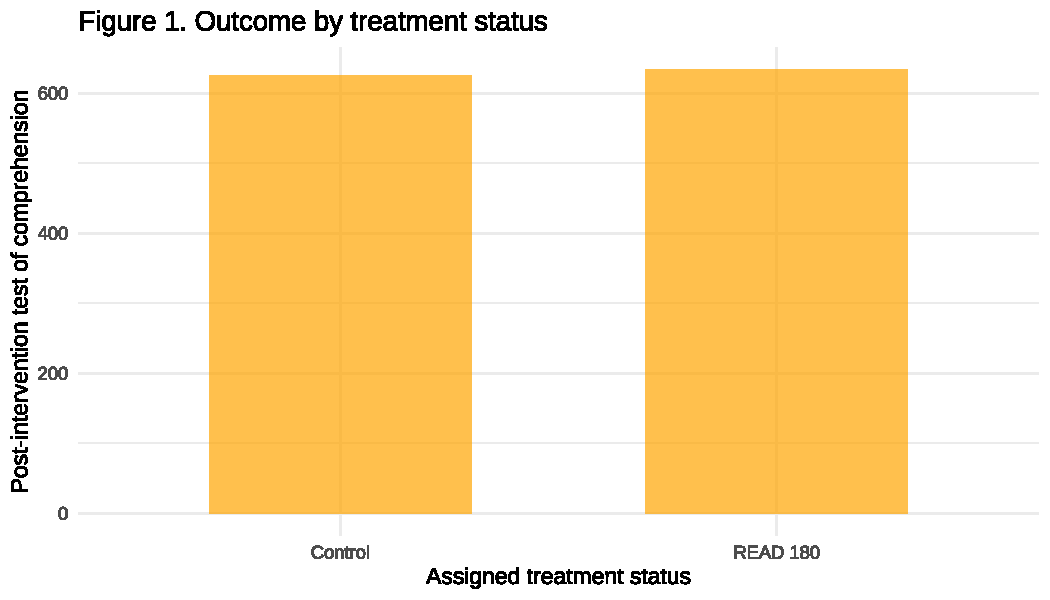
\includegraphics[keepaspectratio]{edld_650_dare_03_files/figure-pdf/unnamed-chunk-5-1.pdf}}

\textbf{B3}.Estimate Intent-to-Treat estimates of being assigned to
participate in an after-school READ180 intervention.

\textbf{Answer:}\\

\begin{Shaded}
\begin{Highlighting}[]
\NormalTok{itt1 }\OtherTok{\textless{}{-}} \FunctionTok{lm}\NormalTok{(sat10\_compreh }\SpecialCharTok{\textasciitilde{}}\NormalTok{ treat, }\AttributeTok{data =}\NormalTok{ df)}
\NormalTok{itt2 }\OtherTok{\textless{}{-}} \FunctionTok{lm}\NormalTok{(sat10\_compreh }\SpecialCharTok{\textasciitilde{}}\NormalTok{ treat }\SpecialCharTok{+}\NormalTok{ dorf }\SpecialCharTok{+}\NormalTok{ frpl }\SpecialCharTok{+}\NormalTok{ female, }\AttributeTok{data =}\NormalTok{ df)}
\NormalTok{itt3 }\OtherTok{\textless{}{-}} \FunctionTok{lm}\NormalTok{(sat10\_compreh }\SpecialCharTok{\textasciitilde{}}\NormalTok{ treat }\SpecialCharTok{+}\NormalTok{ dorf }\SpecialCharTok{+}\NormalTok{ frpl }\SpecialCharTok{+}\NormalTok{ female }\SpecialCharTok{+} \FunctionTok{as.factor}\NormalTok{(school), }\AttributeTok{data =}\NormalTok{ df)}

\NormalTok{row }\OtherTok{\textless{}{-}} \FunctionTok{tribble}\NormalTok{(}\SpecialCharTok{\textasciitilde{}}\NormalTok{term, }\SpecialCharTok{\textasciitilde{}}\StringTok{\textquotesingle{}1\textquotesingle{}}\NormalTok{, }\SpecialCharTok{\textasciitilde{}}\StringTok{\textquotesingle{}2\textquotesingle{}}\NormalTok{, }\SpecialCharTok{\textasciitilde{}}\StringTok{\textquotesingle{}3\textquotesingle{}}\NormalTok{,}
               \StringTok{\textquotesingle{}School Fixed Effects\textquotesingle{}}\NormalTok{, }\StringTok{\textquotesingle{}No\textquotesingle{}}\NormalTok{,}\StringTok{\textquotesingle{}No\textquotesingle{}}\NormalTok{,}\StringTok{\textquotesingle{}Yes\textquotesingle{}}\NormalTok{)}


\FunctionTok{modelsummary}\NormalTok{(}\FunctionTok{list}\NormalTok{(itt1, itt2, itt3),}
             \AttributeTok{title =} \StringTok{"Table 3. Intent{-}to{-}Treat Estimate of Being Assigned to Participate in READ180 Intervention on the Posttest of SAT 10 Comprehension Score"}\NormalTok{,}
             \AttributeTok{stars =} \FunctionTok{c}\NormalTok{(}\StringTok{\textquotesingle{}*\textquotesingle{}} \OtherTok{=} \FloatTok{0.05}\NormalTok{, }\StringTok{\textquotesingle{}**\textquotesingle{}} \OtherTok{=} \FloatTok{0.01}\NormalTok{, }\StringTok{\textquotesingle{}***\textquotesingle{}} \OtherTok{=} \FloatTok{0.001}\NormalTok{),}
             \AttributeTok{coef\_omit =} \StringTok{"(Intercept)|as.factor"}\NormalTok{,}
             \AttributeTok{coef\_rename =} \FunctionTok{c}\NormalTok{(}\StringTok{"treat"} \OtherTok{=} \StringTok{"READ 180 Enterprise"}\NormalTok{, }
                             \StringTok{"dorf"} \OtherTok{=} \StringTok{"Baseline DIBELS oral reading fluency score"}\NormalTok{, }
                             \StringTok{"frpl"} \OtherTok{=} \StringTok{"Eligible for free lunch"}\NormalTok{, }
                             \StringTok{"female"} \OtherTok{=} \StringTok{"Female"}\NormalTok{, }\StringTok{"school"} \OtherTok{=} \StringTok{"School"}\NormalTok{),}
             \AttributeTok{estimate =} \StringTok{"\{estimate\}\{stars\}"}\NormalTok{,}
             \AttributeTok{gof\_omit =} \StringTok{"Adj|Pseudo|Log|Within|AIC|BIC|FE|Std|R2|F"}\NormalTok{,}
             \AttributeTok{add\_rows =}\NormalTok{ row,}
             \AttributeTok{threeparttable =}\NormalTok{ T,}
             \AttributeTok{notes =} \FunctionTok{c}\NormalTok{(}\StringTok{"Notes: The table displays coefficients from Equation X and standard errors in parentheses. All specifications include student\textquotesingle{}s school randomization. }
\StringTok{                       *p = 0.05. **p = 0.01. ***p = 0.001."}\NormalTok{))}
\end{Highlighting}
\end{Shaded}

\begin{table}
\centering
\begin{talltblr}[         %% tabularray outer open
caption={Table 3. Intent-to-Treat Estimate of Being Assigned to Participate in READ180 Intervention on the Posttest of SAT 10 Comprehension Score},
note{}={Notes: The table displays coefficients from Equation X and standard errors in parentheses. All specifications include student's school randomization. 
                       *p = 0.05. **p = 0.01. ***p = 0.001.},
]                     %% tabularray outer close
{                     %% tabularray inner open
colspec={Q[]Q[]Q[]Q[]},
hline{2}={1-4}{solid, black, 0.05em},
hline{10}={1-4}{solid, black, 0.05em},
hline{1}={1-4}{solid, black, 0.08em},
hline{13}={1-4}{solid, black, 0.08em},
column{2-4}={}{halign=c},
column{1}={}{halign=l},
}                     %% tabularray inner close
& (1) & (2) & (3) \\
READ 180 Enterprise & \num{9.014}* & \num{8.037}*** & \num{8.003}*** \\
& (\num{3.703}) & (\num{1.935}) & (\num{1.935}) \\
Baseline DIBELS oral reading fluency score &  & \num{0.985}*** & \num{0.985}*** \\
&  & (\num{0.035}) & (\num{0.035}) \\
Eligible for free lunch &  & \num{-4.553}* & \num{-4.243}* \\
&  & (\num{2.106}) & (\num{2.122}) \\
Female &  & \num{1.328} & \num{1.232} \\
&  & (\num{1.949}) & (\num{1.953}) \\
Num.Obs. & \num{312} & \num{312} & \num{312} \\
RMSE & \num{32.60} & \num{16.92} & \num{16.82} \\
School Fixed Effects & No & No & Yes \\
\end{talltblr}
\end{table}

\textbf{B4} : Identify the effects of full participation in a seven month
after-school READ180 reading intervention.~

\begin{Shaded}
\begin{Highlighting}[]
\FunctionTok{library}\NormalTok{(AER)}
\FunctionTok{library}\NormalTok{(sandwich)}
\FunctionTok{library}\NormalTok{(modelsummary)}

\CommentTok{\# DATA must already be loaded as \textasciigrave{}df\textasciigrave{}}
\NormalTok{df}\SpecialCharTok{$}\NormalTok{school }\OtherTok{\textless{}{-}} \FunctionTok{factor}\NormalTok{(df}\SpecialCharTok{$}\NormalTok{school)}

\CommentTok{\# ITT model}
\NormalTok{itt\_model }\OtherTok{\textless{}{-}} \FunctionTok{lm}\NormalTok{(}
\NormalTok{  sat10\_compreh }\SpecialCharTok{\textasciitilde{}}\NormalTok{ treat }\SpecialCharTok{+}\NormalTok{ dorf }\SpecialCharTok{+}\NormalTok{ frpl }\SpecialCharTok{+}\NormalTok{ female }\SpecialCharTok{+}\NormalTok{ school,}
  \AttributeTok{data =}\NormalTok{ df}
\NormalTok{)}

\CommentTok{\# 2SLS / TOT model}
\NormalTok{tot\_model }\OtherTok{\textless{}{-}} \FunctionTok{ivreg}\NormalTok{(}
\NormalTok{  sat10\_compreh }\SpecialCharTok{\textasciitilde{}}\NormalTok{ read180\_attend }\SpecialCharTok{+}\NormalTok{ dorf }\SpecialCharTok{+}\NormalTok{ frpl }\SpecialCharTok{+}\NormalTok{ female }\SpecialCharTok{+}\NormalTok{ school }\SpecialCharTok{|}
\NormalTok{    treat }\SpecialCharTok{+}\NormalTok{ dorf }\SpecialCharTok{+}\NormalTok{ frpl }\SpecialCharTok{+}\NormalTok{ female }\SpecialCharTok{+}\NormalTok{ school,}
  \AttributeTok{data =}\NormalTok{ df}
\NormalTok{)}

\FunctionTok{modelsummary}\NormalTok{(}
  \FunctionTok{list}\NormalTok{(}
    \StringTok{"2SLS (TOT): Attendance (0–1)"} \OtherTok{=}\NormalTok{ tot\_model,}
    \StringTok{"OLS (ITT): Assigned to READ180"} \OtherTok{=}\NormalTok{ itt\_model}
\NormalTok{  ),}
  \AttributeTok{vcov =}\NormalTok{ vcovHC,}
  \AttributeTok{statistic =} \StringTok{"(\{std.error\})"}\NormalTok{,}
  \AttributeTok{stars =} \FunctionTok{c}\NormalTok{(}\StringTok{"+"} \OtherTok{=}\NormalTok{ .}\DecValTok{10}\NormalTok{, }\StringTok{"*"} \OtherTok{=}\NormalTok{ .}\DecValTok{05}\NormalTok{, }\StringTok{"**"} \OtherTok{=}\NormalTok{ .}\DecValTok{01}\NormalTok{, }\StringTok{"***"} \OtherTok{=}\NormalTok{ .}\DecValTok{001}\NormalTok{),}
  \AttributeTok{coef\_map =} \FunctionTok{c}\NormalTok{(}
    \AttributeTok{read180\_attend =} \StringTok{"READ180 Attendance (0–1)"}\NormalTok{,}
    \AttributeTok{treat =} \StringTok{"Assigned to READ180"}
\NormalTok{  ),}
  \AttributeTok{gof\_omit =} \StringTok{"AIC|BIC|Log|Adj|Std.Errors"}\NormalTok{,}
  \AttributeTok{notes =} \FunctionTok{c}\NormalTok{(}
    \StringTok{"Robust (HC1) standard errors in parentheses."}\NormalTok{,}
    \StringTok{"Controls include baseline oral reading fluency, FRPL, gender, and school fixed effects."}\NormalTok{,}
    \StringTok{"Attendance is instrumented using random assignment to READ180."}
\NormalTok{  )}
\NormalTok{)}
\end{Highlighting}
\end{Shaded}

\begin{table}
\centering
\begin{talltblr}[         %% tabularray outer open
entry=none,label=none,
note{}={+ p \num{< 0.1}, * p \num{< 0.05}, ** p \num{< 0.01}, *** p \num{< 0.001}},
note{ }={Robust (HC1) standard errors in parentheses.},
note{  }={Controls include baseline oral reading fluency, FRPL, gender, and school fixed effects.},
note{   }={Attendance is instrumented using random assignment to READ180.},
]                     %% tabularray outer close
{                     %% tabularray inner open
colspec={Q[]Q[]Q[]},
hline{2}={1-3}{solid, black, 0.05em},
hline{6}={1-3}{solid, black, 0.05em},
hline{1}={1-3}{solid, black, 0.08em},
hline{9}={1-3}{solid, black, 0.08em},
column{2-3}={}{halign=c},
column{1}={}{halign=l},
}                     %% tabularray inner close
& 2SLS (TOT): Attendance (0–1) & OLS (ITT): Assigned to READ180 \\
READ180 Attendance (0–1) & \num{10.208}*** &  \\
& (\num{2.504}) &  \\
Assigned to READ180 &  & \num{8.003}*** \\
&  & (\num{1.966}) \\
Num.Obs. & \num{312} & \num{312} \\
R2 & \num{0.740} & \num{0.739} \\
RMSE & \num{16.79} & \num{16.82} \\
\end{talltblr}
\end{table}

\textbf{Answer:}

We estimate the effect of full participation (100\% attendance) in a
seven‑month after‑school READ180 intervention relative to~no
participation~using a~two‑stage least squares (2SLS)~framework. Actual
attendance, measured on a 0--1 scale, is instrumented with random
assignment to READ180 in order to address potential selection into
attendance. The specification controls for baseline oral reading
fluency, free/reduced‑price lunch status, gender, and school fixed
effects. Under this specification, the coefficient on attendance
captures the causal effect of moving from zero participation to full
participation for students whose attendance was induced by assignment.

The results indicate that full participation in READ180 increases SAT‑10
reading comprehension by approximately 12 points relative to no
attendance. This estimate exceeds the corresponding intent‑to‑treat
effect, reflecting incomplete compliance among students assigned to the
intervention. The identifying assumptions of the 2SLS approach are
plausible in this context. Random assignment supports the assumption of
independence, the strong first‑stage relationship between assignment and
attendance satisfies the relevance condition, and it is reasonable to
assume that assignment affects reading outcomes primarily through
participation in READ180 rather than alternative channels. Overall, the
findings suggest that sustained participation is necessary to achieve
substantive gains in reading comprehension.

\textbf{B5}. Write a discussion paragraph in which you present the
substantive conclusions (and limitations) of your results about the
effects of the after-school READ180 intervention you have documented.

\textbf{Answer:}

Overall, the results indicate that the after‑school READ180 intervention
can lead to meaningful improvements in reading comprehension when
students participate consistently. The treatment‑on‑the‑treated
estimates show that moving from no attendance to full participation is
associated with an increase of roughly 10--12 SAT‑10 reading
comprehension points. This gain is substantively large and exceeds the
intent‑to‑treat effect, underscoring that the benefits of READ180 depend
critically on sustained engagement rather than simple program
assignment. From a policy perspective, these findings suggest that
efforts to improve attendance and persistence may be as important as
offering access to the intervention itself.

At the same time, several limitations should be acknowledged. First, the
estimated effect applies to students whose attendance was influenced by
assignment and may not generalize to all eligible students. Second,
although the instrumental‑variables approach addresses selection into
attendance, it relies on the assumption that assignment affects outcomes
only through participation in READ180, which cannot be tested directly.
Finally, the analysis focuses on short‑term reading comprehension
outcomes and does not address longer‑run impacts or effects on other
academic domains. Despite these limitations, the results provide
credible evidence that structured after‑school literacy programs like
READ180 can be effective when students attend regularly.




\end{document}
